\section{多次反射与当前实际}
\label{sec:5.5}

返地表处有种种未固结物质,诸如水、土壤以及所谓风化带等,这些近地表物质与下面
的石油储集岩层之间的波阻抗差异往往甚为显著,足以产生形形色色的近地表谐振,这些谐
振现象是无法预测的,而且不能用前面几章所述的方法加以解释。

\subsection{硬海底例子}
\label{sec:5.5.1}

图\ref{fig:mltp/multiple}所示是质量极佳的海底多次反射,各双曲线$v^2t^2-x^2
=z_j^2$按均勻间隔$z_j=j\Delta z$出
现,$j=0,1,2......$。除球面发散校正以外,数据未经任何处理。空气比水轻、速度比水层速
度慢,而海底沉积则儿乎总是比水层致密些和速度快一些,这意味着相继出现的多次反射差
不多总是具有交替变化的极性。地震初至的极性通常是模棱两可的,但是此图却波形清晰而
且逐个反射极性交替变化明显可见。相继到达之多次反射的振幅比就是反射系数,图\ref{fig:mltp/multiple}
中的反射系数看来是-0.7左右。多次反射首波(multiply reflected head wave)也
较明显,极性也是一样地交错改变。由于首波的多次反射出现在临界角,它们应具有反射系数
-1.0。我们可见到它们实际是逐级增强的,之所以增强其原因就在于球面扩散校正是以三维传播为基础,
而首波实际是作二维传播的。

就波动理论来说,多次反射是有趣的现象,但是对于地球物理学家,它们却是种严重障
碍,地球物理学家不喜欢见到的携带信息的一次波被多次反射掩盖了。



\begin{figure}[H]
\centering
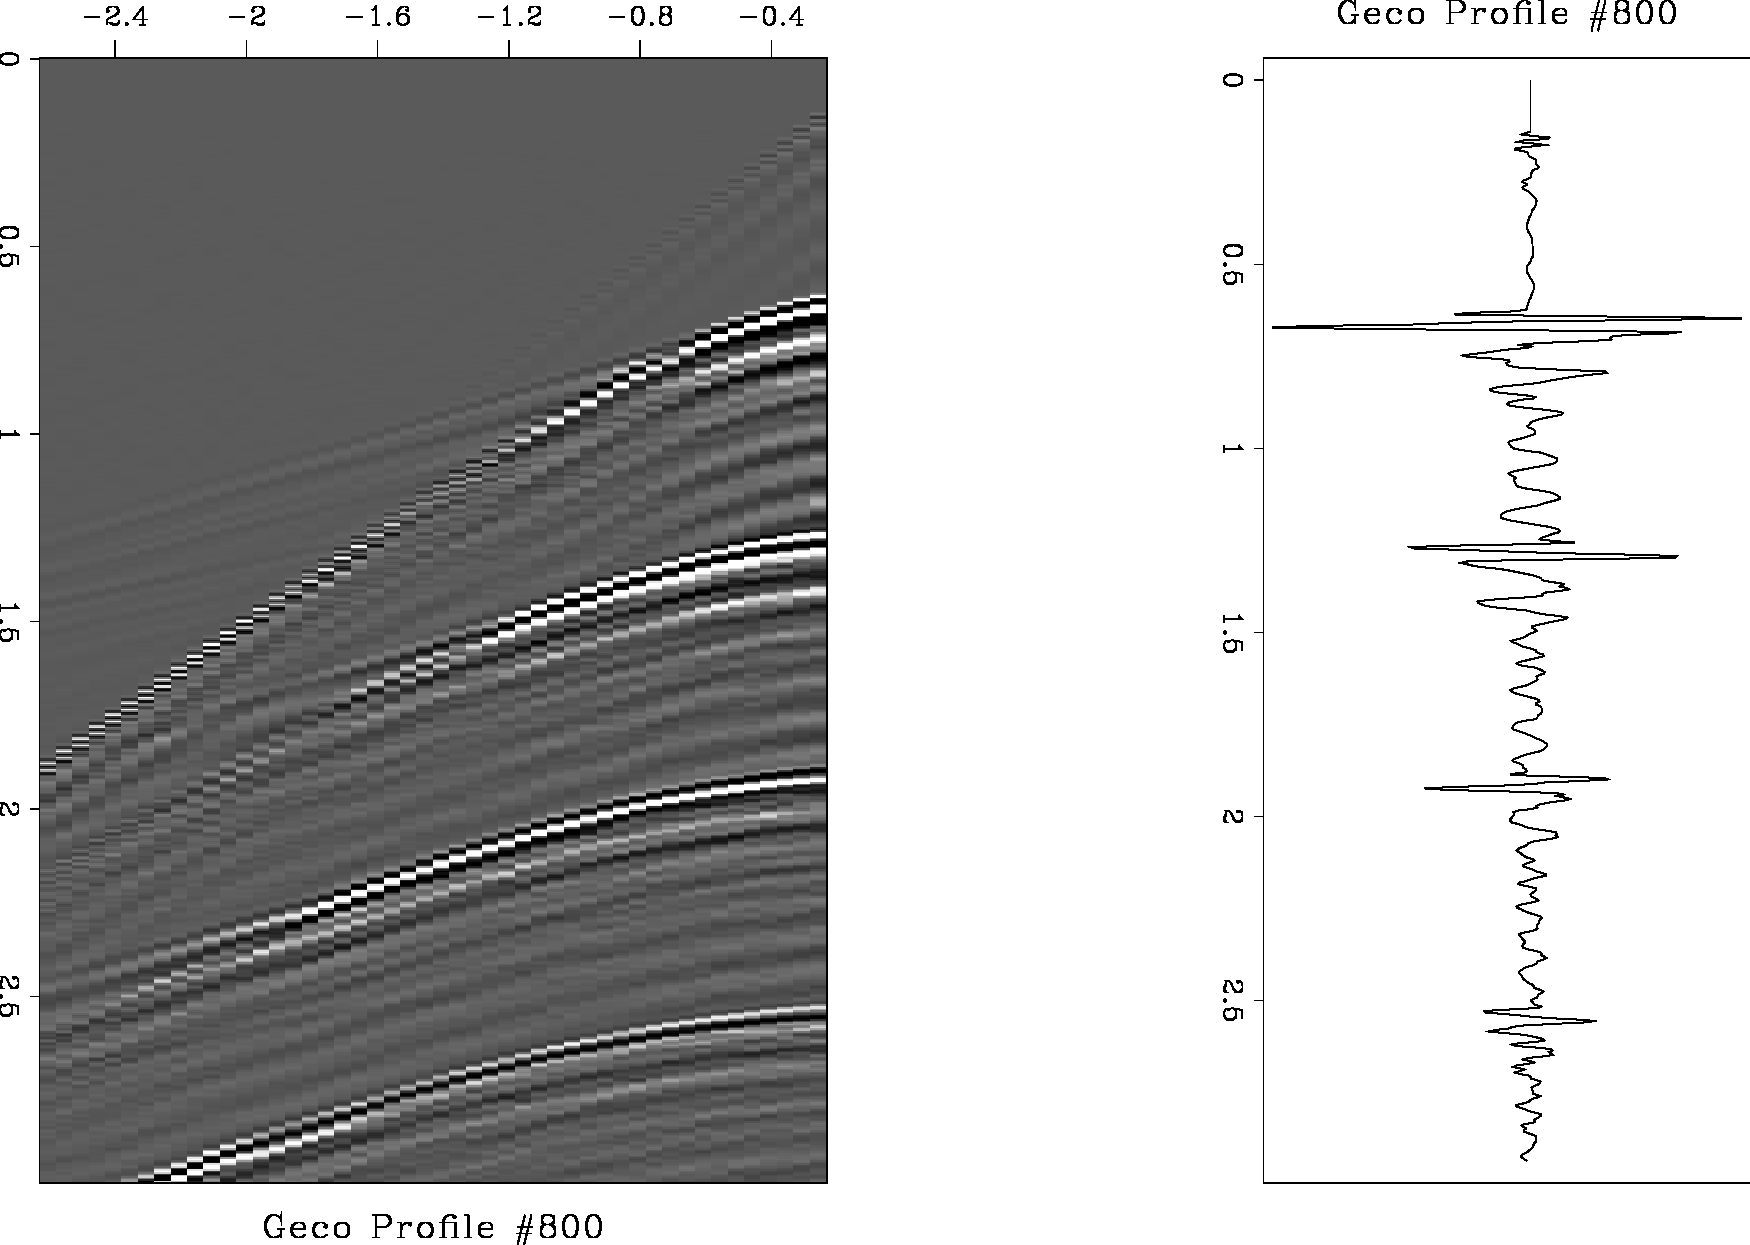
\includegraphics[width=0.65\textwidth]{mltp/multiple}
\caption[multiple]{挪威的多次反射海上剖面。左侧是经过放大的近炮点记录道(据挪威GECO公司)
}
\label{fig:mltp/multiple}
\end{figure}

\subsection{常规数据处理中的反褶积}
\label{sec:5.5.2}

在图\ref{fig:mltp/multiple}中,海水层深度比典型石油勘探深度要大些,图\ref{fig:mltp/gsidecon}与图\ref{fig:mltp/pns}才是更典型的情形。在图\ref{fig:mltp/gsidecon}中,海水层深度浅到不可能辨别出反射了。就陆地资料来说,风化层底部
通常很浅且模糊不清,以致一般不可能识别出单独的反射。“浅”这个字眼R用于多次反射
时是限定只指反射记录变化很迅速,以至没办法钯它们彼此明显区别开来。

\begin{figure}[H]
\centering
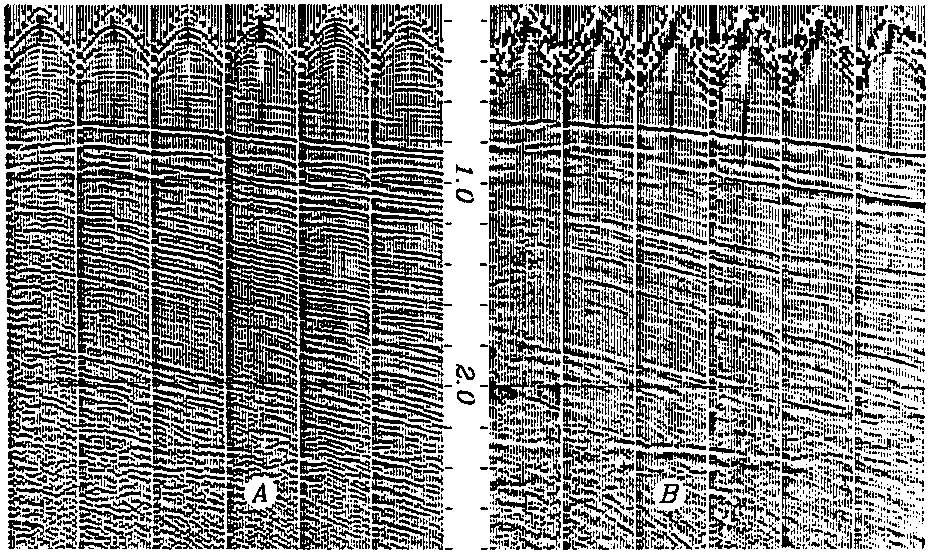
\includegraphics[width=0.65\textwidth]{mltp/gsidecon}
\caption[gsidecon]{
反褶积之前(左图)和反褶积之后(右图)的野外剖面(GSI公司公布,
公元1965年)
}
\label{fig:mltp/gsidecon}
\end{figure}

\begin{figure}[H]
\centering
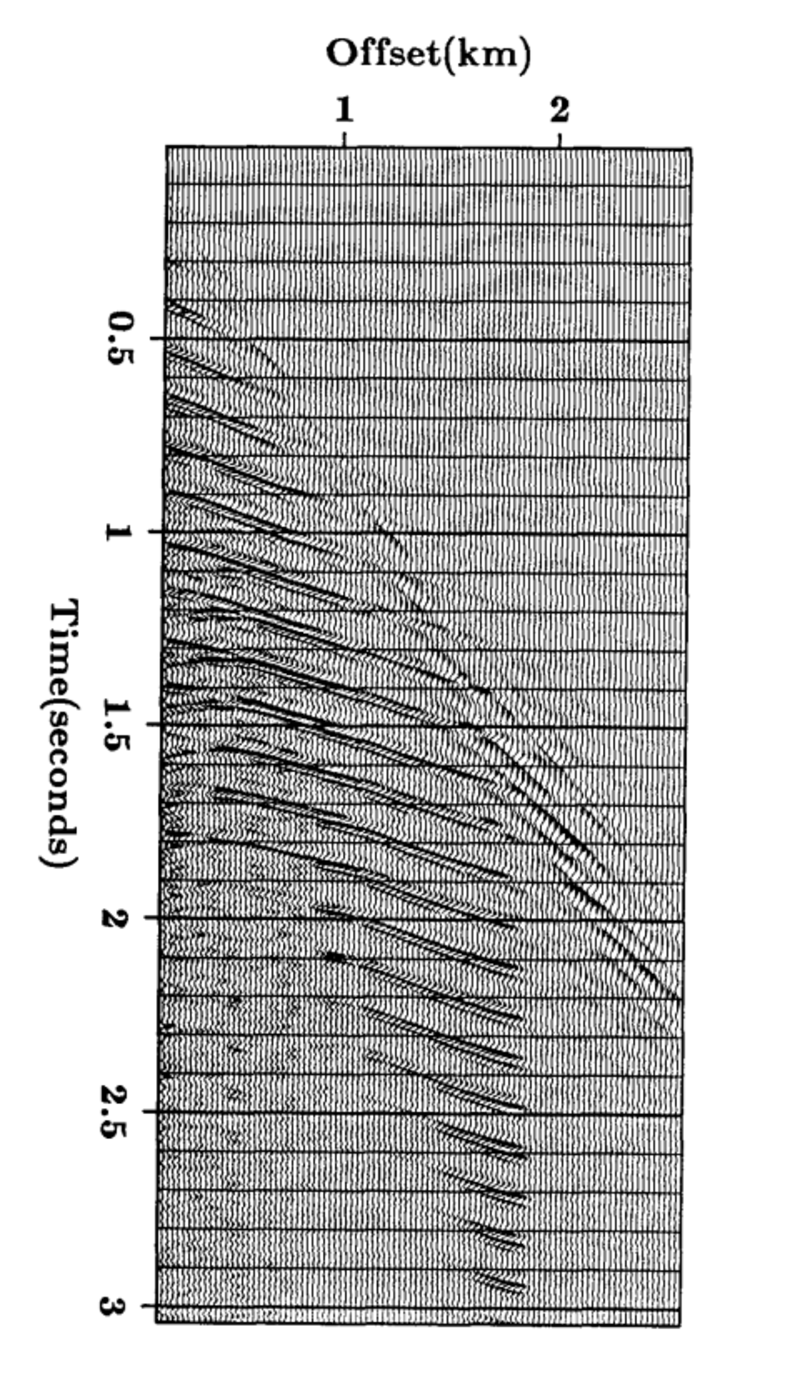
\includegraphics[width=0.65\textwidth]{mltp/pns}
\caption[pns]{
北海剖面(西方地球物理公司)。具有周期大约为90毫秒
之很强的交混回响,它们是海底的多次反射。注意,最强
的信号出现在随时间增长而增大的炮检距上,这是因为最强
的多次波常常在临界角上出现。在船后1.8公里处交混回响
强度突然减低,这是暗示在该点处的海底有突然变化。
}
\label{fig:mltp/pns}
\end{figure}

关于反褶积这个题目,统计学家已经写了一大堆丰富文献了,对于他们来说,这问题实际
是一个估计震源波形而不是消除多次反射的问题。在一定的数学极限之内可使震源波形问題
等价于多次反射问题,当混响只限于炮点或
检波点周围很小的物理体积之内、诸如在土壤
层之内时,这种极限就能成立。震源波形与多
次反射问题之所以能够在这神情形下等价,原
因就在于炮点产生的下行波不但对于炮点本身
来说是固有的,而且也包括了局部土壤层的共
振。在反射地震学中,虚反射这个词是指震源
的反射再加上来自地面的反射(或有时来自风
化层底部),因为震源非常接近这些反射面,
所以我们往往把虚反射也看成是震源波形的一部分。

关于垂直入射情形下的多次反射模型,也
有广泛的文献。在波动传播理论工作者当中,
把消除多次波称作反演问题。看起来,要使反
演理论能应用于实际问题。必须同可处理爆烊
波形未知、频谱性质欠缺问题的分析方法结合起来才行。

常规生产性的反褶积(图\ref{fig:mltp/gsidecon})有许多
种导忠方法积解释,我将以简单的术语来阐述
那些我相信是反褶积之本质的一些问题。每个
地震记录都有一个谱,该谱是许多因素产生的
结果,某些因素具有基本意义,另一些兜j是不增大的炮检距上,这是因为最强的多次波常常在临界角上
重要的。当迆震记录正好因某种近地表现象而
产生共鸣震荡时,这就使人感到麻烦了。反褶积
基本上是这么一种处理:测定出强共鸣震荡,然后设计一种滤波处理去皮制它们。所设
计的滤波具有一种特定的谱,它应大致等于原始数据之谱的倒数,因而,滤波的输出大致为
白噪(所有频率成分均相等)。从最早期开始,地震学家就已经发现反射地震数据在10至
100赫兹频带之外很少有多大意义,所以采取的最后一个步骤就是将该频带范围之外的频率
成分均消除。(对大多数地震学家来说,关于输出的谱应为白噪的假设看来是一稗不得已的
假设,但是实践通常都表明,比起从原始数据来解释地层映象,那它还是更可取的)。

关于反褶积在实践中为什么成功还有另一种非数学的解释,这就是,它使谱逐道相等了,
它实现了各个谱的均衡(Tufekcic等,1981)。不但迆震记录因某科近地表现象而出现共振
是件烦扰的事,而且波谱随近地表条件之逐点变化而出现逐道变化,更是一件令人头痛的
事,变化的波谱使得时差的测定很难进行。要注意,以上所述的常规生产性反褶积处理就是
将谱均衡(spectral balancing)作为一种副产品包括在内的。图\ref{fig:mltp/pns}所示就是需要进行
谱均衡的数据。

上述对反褶积及其为何能起作用的解释不同于大多数地球物理文献中所作的解释,通常
总是用多次反射可预测而一次反射不可预测来解释反褶积。在《地球物理数据处理基础》一
书中指出过如何预测多次反射,它们不是采用严格的褶积模型,而只不过是近似迆采用该模
型来预测多次反射。只有当交混回响全部存在于浅层中时,基于褶积模型的预测才起最佳作
用。这时,交混回响丨象是一个震源波形。

心血管研究须很好地与日常实践结合起来,而肺功能研究则否。我认为这点与下述事实
可相比拟:偏移理论与速度理论是生产实践的良好指南,而反褶积理论则不然。理论与实践
之间留有较大之空白,意味着还存在有某种有待认识的事物。某些领域很难直接着手解决,
在这些领域中,你必须循着更迂迴的间接途径前进,学生会被这弄糊涂,而缺乏耐心的人则
会感到混乱,但是,仅此途径,别无他法。欲悉详情,可阅ZioIkowski(1984)的著作。

下面将用少量篇幅指出,采用井中检波器的陆地资料进一步证实震源波形主耍就是近地
表交混回响;然后离开褶积模型,转而讨论其它。

\subsection{垂直地震剖面(VSP)}
\label{sec:5.5.3}

地震学家总是欢迎垂直地震剖面的额外信息。VSP是震源在地面、由井中检波器记录所
得地震记录的某种组合,诸如岩屑和电测井等常规以井为基础的观测都是记录局部信息,影
响所及范围距井壁不过几公分。把地层考虑为水平成层倒是不错,但就是距井壁为某种未知
距离之处这种理想化情形并不成立。反射勘探地震学尽管离钻井观测的“可靠真理”还差得
远,仍能提供关于横向连续性所需要的信息,但是地面观测反射资料既受分辨能力限制,又
有其他不肯定性响影。VSP提供中等比例尺度的信息,而且还为地面地震方法提供一种标定
办法,可惜的是,VSP方法的费用昂贵,因而我们很难得到VSP数据。

关于VSP这个题目已有若干专著和许多研究论文(见Gal'perin,1974及Balch等,1982),
在这里我们将只考虑一个VSP记录,以便得出震源波形及多次反射的某些概念。图\ref{fig:mltp/vspl}所
示VSP剖面取自典型的陆地区域,多次反射影响不如本章其他处所示海上资料那么严重。图
\ref{fig:mltp/vspl}中最早到达的波至是一次下行波。下行波旅行时间随深度而増大,时距曲线之斜率给
出向下速度分量。在第一个下冇波到达以后,你可见有更多的具有相同速度之下行波。上行
波具有与下行波符号相反的斜率,这些波在图\ref{fig:mltp/vspl}内亦明显可见。
\begin{figure}[H]
\centering
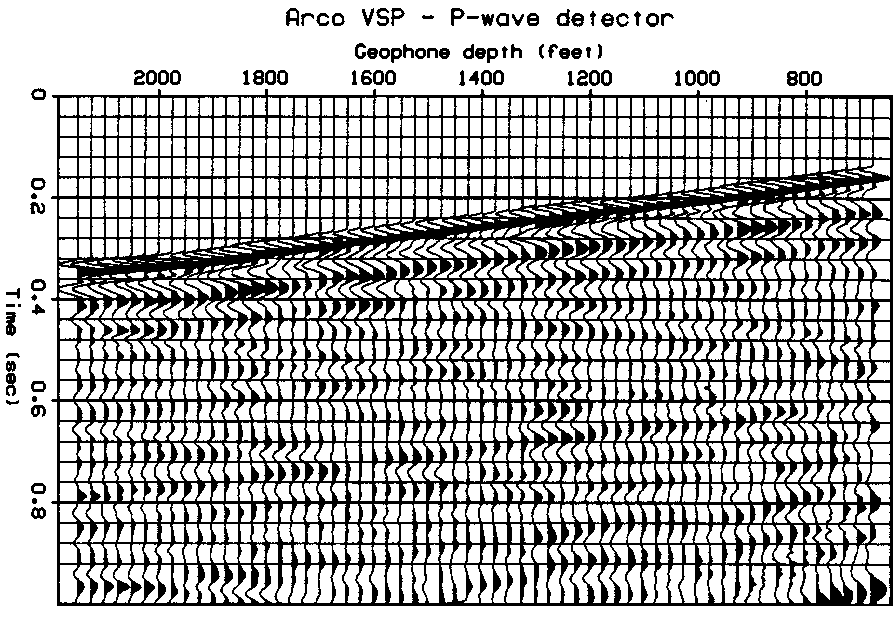
\includegraphics[width=0.65\textwidth]{mltp/vspl}
\caption[vspl]{
垂直地震剖面。震源位于钻孔附近地表面,水平轴为接收器深度,垂直轴为
从零至一秒的旅行时间。振幅均按$t^{1.5}$作比例标定(ARCO公司)
}
\label{fig:mltp/vspl}
\end{figure}

由于晚到的反射弱于早到的硖,地震资料在进行显示之前通寧要辨时间而加以比例
标定,关于什么比例标定最好的问题,无论在理论上或实践中都没有什么通用规定。通常,我
发现按$t^2$进行标定可使反射资料令人满意(见\ref{sec:4.1}节)。图\ref{fig:mltp/vspl}表明,按$t^{1.5}$进行标定可保
持VSP剖面上的初至大体为恒定振幅。

从侧面仔细观察图\ref{fig:mltp/vspl}可发现,下行脉冲后面跟随有一逐个深度均有几分一致的波形,
一致的程度因上行波干涉而不易看出.就我由该图所能告诉你的是,最大深度处的下行波等
于最浅深度处的下行波。

图\ref{fig:mltp/vsp2}所示是相同资料,但系将某些浅层接收点所得结果加以増强而成。你会注意到,下
朽波看来不再是与深度无关了。因此,我们可以得出结论,就实际问题而论,下行波的波形
似乎主要是近地表交混回响形成的一个结果。
\begin{figure}[H]
\centering
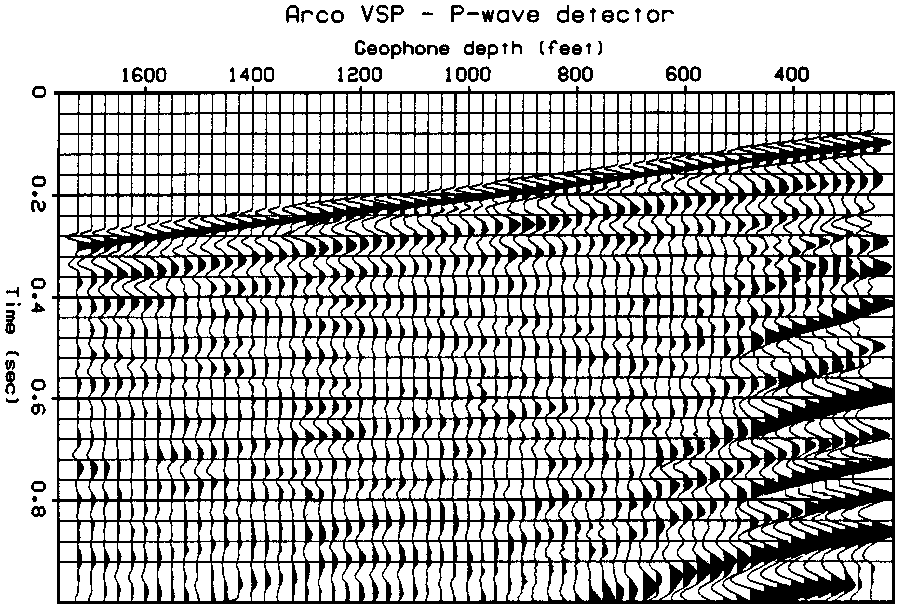
\includegraphics[width=0.65\textwidth]{mltp/vsp2}
\caption[vsp2]{
图\ref{fig:mltp/vspl}的数据按浅层接收点增强而得的结果。振幅
均按$t^{1.5}$作比例标定(ARCO公司)
}
\label{fig:mltp/vsp2}
\end{figure}

图\ref{fig:mltp/vspl}中第一个脉冲的能量大体可与其余脉冲能量相比拟,如果VSP的显示不采用
$t^{1.5}$进行比例标定,其余能量就会小一些,但是既然地面反射资料通常都用某些这类比例标
定(往往是采用$t^2$
),这就使得从统计的角度谈论标定数据中的能量变得更有意义了。所
以,交混回响能量是大体可与初至能量相比拟的。

在近地表区域以下,下行波随深度而缓慢变化。我们现在要问:如将排列横向移动的
话,下行波究竟会变化多少。显然,钻井不会横向移动,因而我们将局限于仅是地面震源横
向移动情形下的记录数据。由于近地表变动往往在横向上迅速改变,我们也许要担心下行波
波形也是随炮点位置而迅速变化。炮点附近的交混回响同任何地面接收器附近的馄响是类似
重复的,最终组成的交混回响就是近炮点交混回响与近检波点交混回响二者的摺积。因此,
为获得对地面垲震数据进行反褶积时所需要的信息,VSP应当利用许多地面震源位置进行记
录。

可惜,这样的非零炮检距VSP资料难得采用。当石油生产下降因而打算采用费用昂贵的
二次回采方法时八VSP的成本费用相比起来就不会显得那么高了;
VSP观测期间停止生产的
损失与未来的利润收益二者之间孰轻孰重是很容易掂量出来的。

再有,我们应当思考一下所谓“坏”资料的意义。地震数据每当高于周围环境微地震干
扰的水平时,一般总是可重复的。但是往往信号却毫无意义,空间相关对我们来说无
关轻重。大多数资料在较大时间时的情形都适于这样描述,出现的问题或许是下列这些:
(1)下行波波形拖有一个很长的尾巴;(2
)尾巴是地面位置的某种无序函数(chaotic function );(3
)尾巴的能量超过第一个脉冲的能量。因此,由于下行波内有如此之多的
随机性,上行波必然是难以理解的。

\subsection{深海多次皮---极地纬度的现象}
\label{sec:5.5.4}

有一种经常引人注意的事,即,海底多次反射似乎大都只在极地纬度才是问题,难得在
赤道区域内出现。由于所根据的统计资料不多,这种观察也许有不妥之点,不过有两个理由
可以解释为什么这种观察窄可能成立,无论统计数字是否适当,它们每个都具有意义。

天然气往往可溶化于水,因而提高了凝固温度,在高压下尤其如此;当存在天然气时形
成的冰,称为天然气水化物(gas hydrate),因此,在液体海洋之下可能存在有圈闭于沉
积物之内的固体天然气水化物,该天然气水化物使沉积物的刚度増大,从而増强了多次反
射。

关于在极地纬度地区出现强多次反射的第二个理由一定与冰蚀作用有关。海洋底部普通
都是慢速沉积细粒物质的场所,这类新沉积的岩层均较柔软,故可形成弱多次反射波;但是
在极地纬度地区,冰川的冲蚀作用将沉积物搬运走了,在发生侵蚀的地方,新剥露出的岩石
比新近形成的沉积物强固坚硬。因此形成了较强的反射。

大陆在所有纬度上都会有侵蚀和沉积,然而,人们可以推测,在平衡时,在低纬度和中
等纬度地区的沉积作用形成了大陆斜坡,以后漂移至高纬度地区,在那里它们被侵蚀了。尽
管这很大程度上是推测想象,但这种理论确实为多次反射与极地纬度有关的原因提供了一种
解释。

\subsection{微屈多次反射与层内多次反射}
\label{sec:5.5.5}

所有多次反射类型均不出图\ref{fig:mltp/multpath}所示三类基本范畴之一。

\begin{figure}[H]
\centering
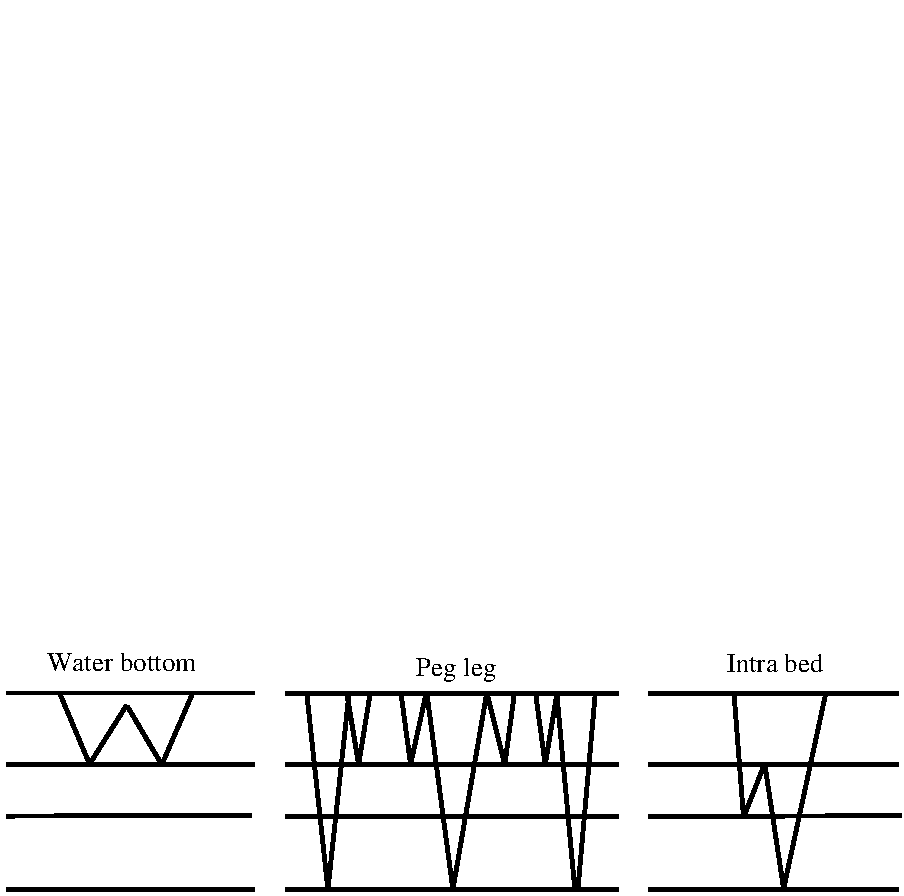
\includegraphics[width=0.65\textwidth]{mltp/multpath}
\caption[multpath]{
所示射线路程分别为(a)海底多次波(b)微屈多次波(c)短程多次波
}
\label{fig:mltp/multpath}
\end{figure}

海底多次波是射线路程整个位于海水层内部的那些多次波,如图\ref{fig:mltp/multpath}(a),由于海底通常
具有比深地质层位为高的反射率,海底多次波往往有很强振幅。在深水中,这些多次波可能
非常明显,截然不同,图\ref{fig:mltp/nearoffset}中所示是这类多次波的一个范例。

\begin{figure}[H]
\centering
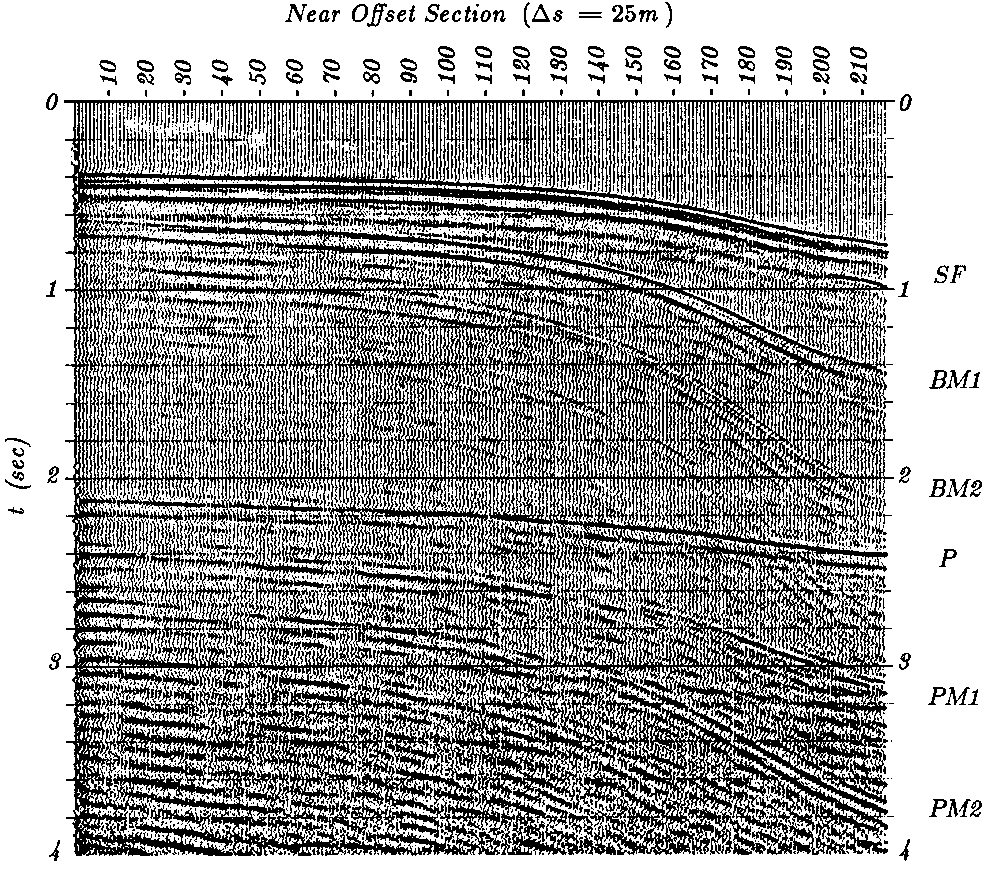
\includegraphics[width=0.65\textwidth]{mltp/nearoffset}
\caption[nearoffset]{
近炮检距剖面---近海拉长石Flemish顶板岩层。
炮检距的距离约为9个炮点之距离,为海底,SF为第一个海底多次反射,BM2为第二个海底多次反
射。P为一次波,PMl为第一个微屈多次波,PM2为第二个微屈多次波(AMOCO-Canada公司)
}
\label{fig:mltp/nearoffset}
\end{figure}

微屈多次反射按不同的作者有种种不同的定义,图\ref{fig:mltp/multpath}(b)中将微屈多次波定义为有
一次在沉积层系内发生反射而其他反射均在近地表发生的那些多次波。

为便于解释地震资料,让我们回顾一下层状介质内垂直入射多次反射的时间与振幅关
系。取海底反射系数为$c_1$,双程旅行时间为$t_1$,则第n次多次反射在时间$nt_1$到达,反射强度
为$c_1^n$;再假设较深层的一次反射旅行时间深度为$t_2$,具有反射系数$c_2$,于是海底微屈多次波
是在时间$t_2+nt_1$到达。注意,微屈多次波应成群到达,例如,时间$t_2+2t_1$可由三种路程所
形成,即$t_2+2t_1$、$t_1+t_2+t_1$或$2t_1+t_2$。因此,n阶微屈多次回声反射实际是来自n+1种射
线路程之反射的总和,从而其强度与$(n+1)c_2c_1^n$
成比例。海底混响的强度为这点同描述
沉积地层发生过一次反射混响时采用$(n+1)c_1^n$那样的n之函数是不相同的,忽略海底交混
回响本身,你可以仅把$(n+1)c_1^n$当作是爆炸波形。

每种多次波必然都有上行波变为下行波的“回车换向”点,儿乎所有容易识别的多次波
都是垲面多次波,就是说,它们的换向点均在地表,图\ref{fig:mltp/nearoffset}所示就是一些明显的例子,在
陆地勘探资料中,回车换向点可以是在土壤层底部,这差不多就同位于地表是一回事。

代表另一类称为“短程”多次波或“层内”多次反射波的射线路程,如图\ref{fig:mltp/multpath}
(c)所
示,它们的换向点不在地表或不接近地表。在野外资料中,这类多次波极少是明显可见的,
尽管图\ref{fig:mltp/intrabed}所示是一种很清楚的情形,其中的这类多次波就不大容易看出来。它们能被追
踪识别,往往是因为地震资料是利用一些附带的测井记录进行综合解释的结杲,与微屈多次
波相比,这类短程多次波如此难以观察到的原因就在于:沉积层系内部的反射系数比自由面
上的反射系数低很多,不过,短程多次波的这个弱点可以被它们可能出现的次数非常之大所补
偿。不论任何时候,只要地震剖面变得难以解释,我们就可假定资料准是己变得以短程多次
波占压倒优势了。

\begin{figure}[H]
\centering
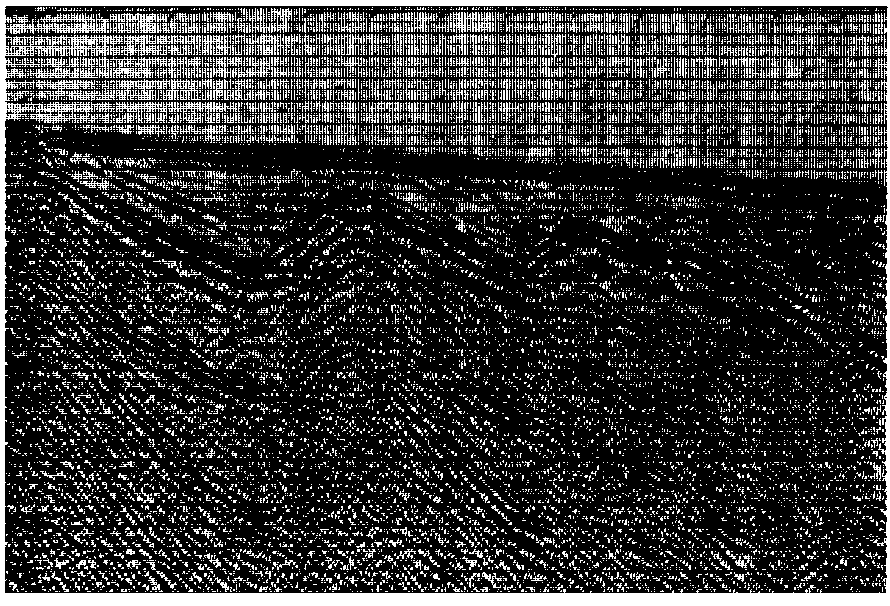
\includegraphics[width=0.65\textwidth]{mltp/intrabed}
\caption[intrabed]{
有确凿之层间多次反射的罕有情形
资料系在波多黎各附近记录到,层内多次波处于海底反射与基底反射之间,因而其旅行时间为
$t_{base}+(t_{base}-t_{floor})$,你看出它没有?(据西方地球物理公司)
}
\label{fig:mltp/intrabed}
\end{figure}

\subsection{对各种剖面类型需有所区别}
\label{sec:5.5.6}






